	%-=-=-=-=-=-=-=-=-=-=-=-=-=-=-=-=-=-=-=-=-=-=-=-=
%
%        LOADING DOCUMENT
%
%-=-=-=-=-=-=-=-=-=-=-=-=-=-=-=-=-=-=-=-=-=-=-=-=

\documentclass[newPxFont,pagenumber]{beamer}
\usetheme{sthlm}
%\usecolortheme{sthlmv42}

%-=-=-=-=-=-=-=-=-=-=-=-=-=-=-=-=-=-=-=-=-=-=-=-=
%        LOADING PACKAGES
%-=-=-=-=-=-=-=-=-=-=-=-=-=-=-=-=-=-=-=-=-=-=-=-=
\usepackage[utf8]{inputenc}
\usepackage[frenchb]{babel}
\usepackage[normalem]{ulem}
\usepackage{caption}
\captionsetup{font=scriptsize}
%\usepackage[font=footnotesize]{subcaption}
% in preamble
\usepackage{chronology}
\usepackage{pgf}
\usepackage[linesnumbered,ruled,vlined]{algorithm2e}
\usepackage{tikz}
\usetikzlibrary{arrows,automata}
\usepackage{array,multirow}
\usepackage{nameref}
\usepackage{xcolor}
\definecolor{shadecolor}{RGB}{51,51,51}

\makeatletter
\newcommand*{\currentname}{\@currentlabelname}
\makeatother

\graphicspath{ {fig/} }
% add page number
%\usepackage[defaultsans]{cantarell}

\newcommand{\p}{\mathbb{P}}

\setbeamerfont{title}{series=\upshape}
\setbeamertemplate{footline}{\hfill\footnotesize\insertframenumber\hskip3pt\null\vskip3pt}

\newcommand{\argmax}{\mathop{\mathrm{argmax}}\limits}
\renewcommand{\max}{\mathop{\mathrm{max}}\limits}

\renewcommand{\event}[3][e]{%
  \pgfmathsetlength\xstop{(#2-\theyearstart)*\unit}%
  \ifx #1e%
    \draw[fill=black,draw=none,opacity=0.5]%
      (\xstop, 0) circle (.2\unit)%
      node[opacity=1,rotate=45,right=.2\unit] {#3};%
  \else%
    \pgfmathsetlength\xstart{(#1-\theyearstart)*\unit}%
    \draw[fill=black,draw=none,opacity=0.5,rounded corners=.1\unit]%
      (\xstart,-.1\unit) rectangle%
      node[opacity=1,rotate=45,right=.2\unit] {#3} (\xstop,.1\unit);%
  \fi}%

\addto\captionsfrench{%
\renewcommand{\figurename}{\scriptsize {\scshape Figure}}
\renewcommand{\tablename}{\scriptsize {\scshape Table}}
}

%-=-=-=-=-=-=-=-=-=-=-=-=-=-=-=-=-=-=-=-=-=-=-=-=
%        BEAMER OPTIONS
%-=-=-=-=-=-=-=-=-=-=-=-=-=-=-=-=-=-=-=-=-=-=-=-=

%\setbeameroption{show notes}

%-=-=-=-=-=-=-=-=-=-=-=-=-=-=-=-=-=-=-=-=-=-=-=-=
%
%	PRESENTATION INFORMATION
%
%-=-=-=-=-=-=-=-=-=-=-=-=-=-=-=-=-=-=-=-=-=-=-=-=

\title{\large Méthodes D'Analyse Sémantique De Corpus De Décisions Jurisprudentielles}
\subtitle{\scriptsize Soutenance de thèse de doctorat en informatique de l'IMT Mines Alès}
%\date{\small{\jobname}}
%\date{\scriptsize Début de thèse: 15 Décembre 2015}
\date{\scriptsize 24 janvier 2020}
\author{\small Gildas TAGNY NGOMPÉ}
\institute{\tiny \textbf{Jury:} \begin{itemize}
\item Stéphane MUSSARD, Professeur, Université de Nîmes (Directeur de thèse)
\item Jacky MONTMAIN, Professeur, IMT Mines Alès (Co-directeur de thèse)
\item Sandra BRINGAY, Professeur, Université Paul Valéry Montpellier (Rapporteur)
\item Mohand BOUGHANEM, Professeur, Université Toulouse III Paul Sabatier (Rapporteur)
\item Françoise SEYTE, Maître de Conférences (HDR), Université de Montpellier (Examinateur)
\item Fabrice MUHLENBACH,  Maître de Conférences, Université Jean Monnet de Saint-Étienne (Examinateur)
\item Guillaume ZAMBRANO, Maître de Conférences, Université de Nîmes (Encadrant de proximité)
\item Sébastien HARISPE,  Maître Assistant, IMT Mines Alès (Encadrant de proximité)
\end{itemize}}

\hypersetup{
pdfauthor = {\author{}: tagnyngompe@gmail.com},
pdfsubject = {},
pdfkeywords = {},
pdfmoddate= {D:\pdfdate},
pdfcreator = {}
}

\begin{document}
\nocite{}
%-=-=-=-=-=-=-=-=-=-=-=-=-=-=-=-=-=-=-=-=-=-=-=-=
%
%	TITLE PAGE
%
%-=-=-=-=-=-=-=-=-=-=-=-=-=-=-=-=-=-=-=-=-=-=-=-=
\begin{frame}[plain]
	\titlepage
\end{frame}
%}
%-=-=-=-=-=-=-=-=-=-=-=-=-=-=-=-=-=-=-=-=-=-=-=-=
%
%	TABLE OF CONTENTS: Plan
%
%-=-=-=-=-=-=-=-=-=-=-=-=-=-=-=-=-=-=-=-=-=-=-=-=
\section*{Plan}
\begin{frame}[c]{\currentname}
\tableofcontents[hideallsubsections]
\end{frame}

\section{Introduction}

\begin{frame}[c]{Les juristes analysent les décisions}
	\begin{center}
		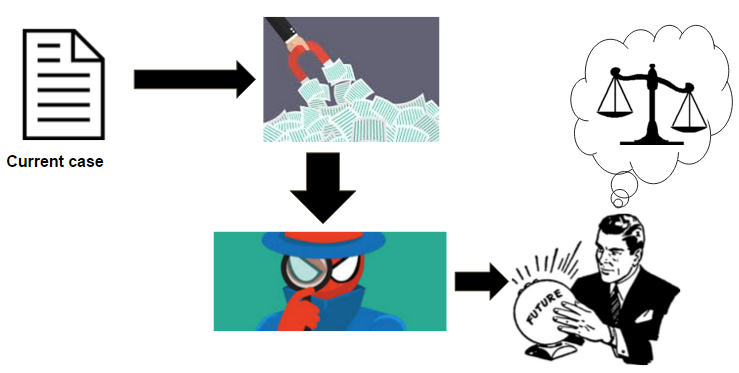
\includegraphics[width=0.7\textwidth]{lawyerwork.png}
	\end{center}
	
	\begin{block}{Pourquoi?}
		\begin{itemize}
			\item comprendre et comparer l'application loi (contentieux, ville, ...)
			\item estimer le risque judiciaire
			\item ... %anticiper les affaires futures
		\end{itemize}
	\end{block}
\end{frame}

\begin{frame}{Motivation: documents non-structurés, langage complexe}
	\scriptsize
	\begin{columns}
		\begin{column}{.50\linewidth}
			ARRÊT N°
			
			R.G: 11/03924
			
			...
			
			{COUR D'APPEL} DE {NÎMES}
			
			{CHAMBRE CIVILE}
			
			{1ère Chambre A}
			
			ARRÊT DU {20 MARS 2012}
			
			APPELANTE:
			
			{Madame Michéle A.} ...
			
			assistée de la {SELARL VAJOU}, ...
			
			INTIMES:
			
			{Monsieur Martial B} ...
			
			assisté de la {SCP MARION GUIZARD PATRICIA SERVAIS}, ...
			
			COMPOSITION DE LA COUR LORS DU DÉLIBÉRÉ:
			
			{M. Dominique BRUZY, Président}
			
			{M. Serge BERTHET, Conseiller}
			
			...
		\end{column}
		\begin{column}{.50\linewidth}
			FAITS, PROCEDURE, ...
			
			Madame Michèle A. demande:
			
			...
			
			- de condamner Madame JONES-B. à lui payer la somme de {2.500 euros} au titre de l'{article 700 du Code de Procédure Civile}, 
			
			\vspace{0.4cm}
			
			PAR CES MOTIFS, LA COUR:
			
			...
			
			Vu l'{article 809 du Code de Procédure Civile},
			
			...
			
			{Déboute Madame A. de sa demande de provision sur dommages-intérêts.}
			
			...
			
			Vu l'{article 700 du Code de Procédure Civile},
			
			Condamne Madame JONES-B. à verser à Madame A. la somme de {2.500 euros}.
		\end{column}
	\end{columns}
\end{frame}

\begin{frame}[c]{Motivation: grand volume de décisions}
	\textbf{Plus de 4 millions de décisions prononcées / an}
	\begin{table}[!htb]
		\scriptsize
		\begin{center}
			\begin{tabular}{|l|l|l|l|l|l|}
				\hline
				\textbf{Justice}	& \textbf{2013}  & \textbf{2014}  & \textbf{2015}  & \textbf{2016}  & \textbf{2017}  \\ \hline
				civile   & 2 761 554 & 2 618 374 & 2 674 878 & 2 630 085 & 2 609 394 \\ \hline
				pénale   & 1 303 469 & 1 203 339 & 1 206 477 & 1 200 575 & 1 180 949 \\ \hline
				administrative & 221 882 & 230 477 & 228 876 & 231 909 & 242 882 \\ \hline
			\end{tabular}
			
			\textit{\scriptsize{\textbf{Source}: \url{http://www.justice.gouv.fr/statistiques-10054/chiffres-cles-de-la-justice-10303/}}}  
		\end{center}
		\caption{Nombre de décisions prononcées en France par an de 2013 à 2017.}\label{tab:intro:nbdecisionstats}
	\end{table}
\end{frame}

\begin{frame}[t]{Motivation: recherches et analyses sémantiques difficiles}
	
	Moteurs de recherche juridique à mots-clés 
	
	Aucune analyse synthétique des décisions 
	
	%\begin{figure}
	\fbox{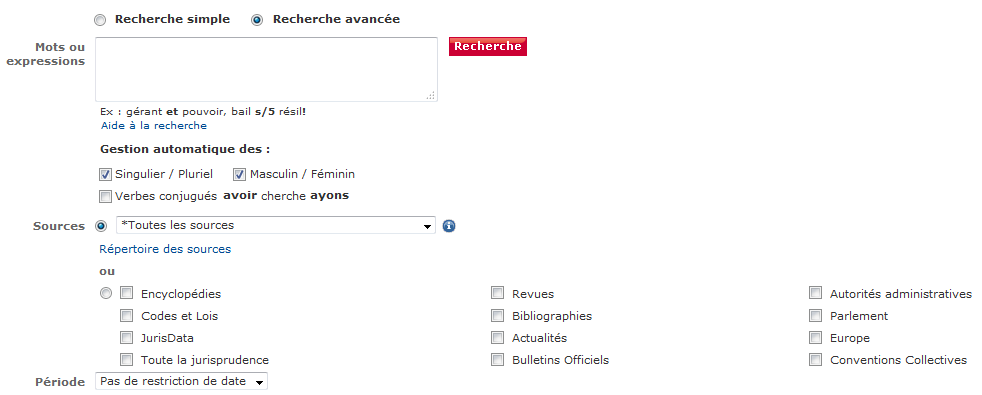
\includegraphics[width=0.9\paperwidth]{jurica.png}}
	
	\textit{\tiny{Source: \url{LexisNexis.com}}} 
	%\caption{Formulaire de recherche}
	%\end{figure}
\end{frame}

\begin{frame}[c]{Objectif : automatiser des tâches d'analyse de décisions}
	\only<1>{\begin{figure}[!htb]
		% pipeline-cassandra.pdf
		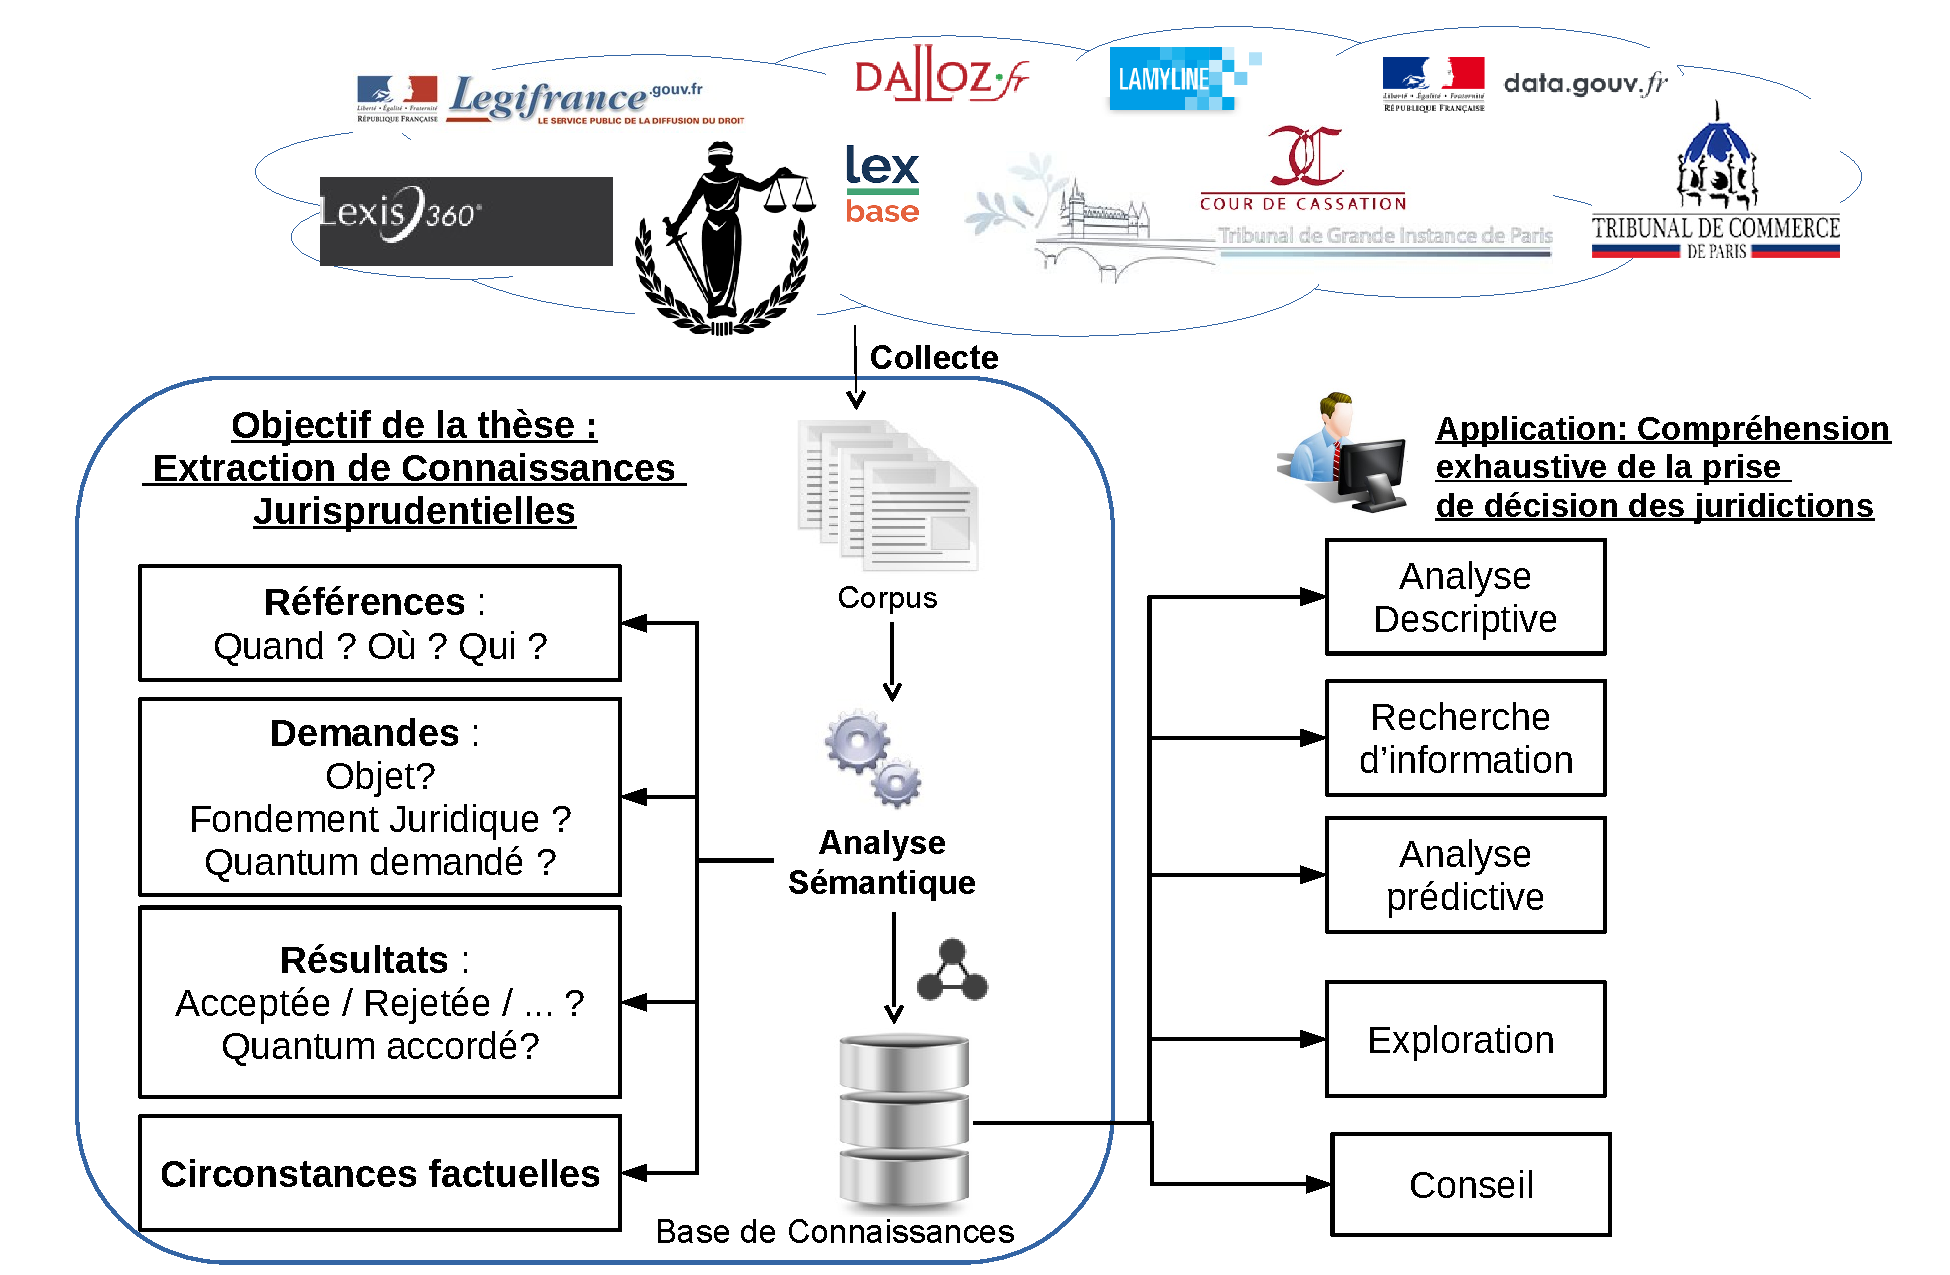
\includegraphics[width=\textwidth]{Objectif_these.pdf}
		\caption{Objectifs et exemples d'application de la thèse.} \label{fig:intro:objectif-these}
	\end{figure}}

	\only<2>{\begin{figure}[!htb]
		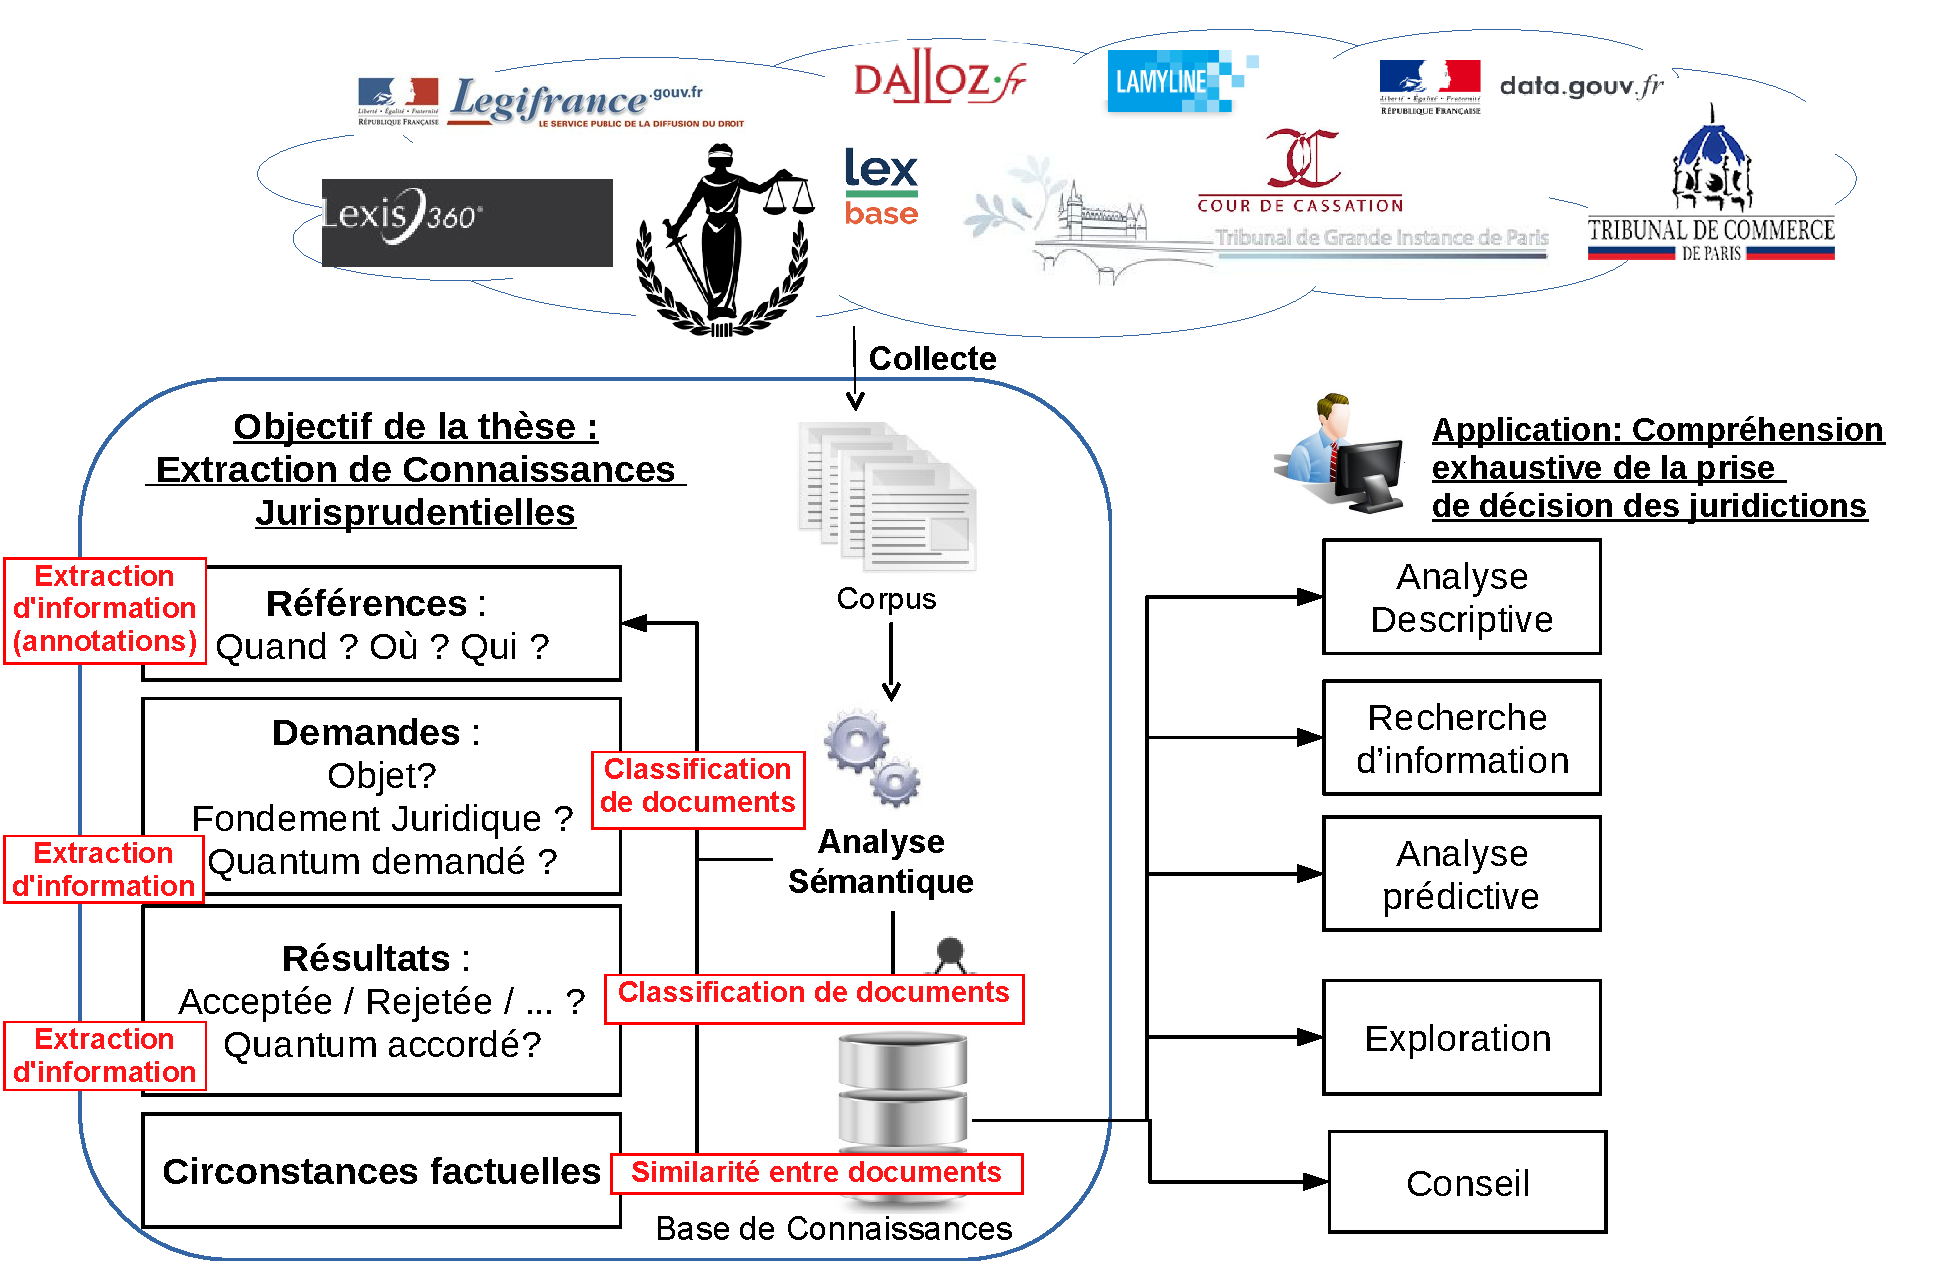
\includegraphics[width=\textwidth]{Objectif_these-problemes2.pdf}
		\caption{Objectifs et problèmes correspondants en analyse de données textuelles.} \label{fig:intro:objectif-these-problemes}
	\end{figure}}
\end{frame}

\begin{frame}[c]{Problème : annotation de sections, métadonnées, normes}
	\[idf(t) = \log_2\left(\frac{N}{N_t}\right)\]
\end{frame}

\begin{frame}[c]{Problème : extraction des demandes}
	
\end{frame}

\begin{frame}[c]{Problème : découverte des circonstances factuelles}
	
\end{frame}

\section{Analyse automatique des corpus judiciaires}

\begin{frame}[c]{Annotation et extraction d'information}
	
\end{frame}

\begin{frame}[c]{Classification de documents}
	
\end{frame}

\begin{frame}[c]{Similarité entre texte}
	
\end{frame}


\section{Contributions}
\begin{frame}[c]{Application du HMM et du CRF pour l'annotation}
	\only<1>{1. Méthodes}
	\only<2>{2. Résultats}	
\end{frame}


\begin{frame}[c]{Retrouver les demandes à l'aide des termes clés}
	\only<1>{1. Méthodes}
	\only<2>{2. Résultats}		
\end{frame}

\begin{frame}[c]{Extension du Gini-PLS pour la classification de textes}
	\only<1>{1. Méthodes}
	\only<2>{2. Résultats}		
\end{frame}

\begin{frame}[c]{Apprentissage de la similarité par transformation}
	\only<1>{1. Méthodes}
	\only<2>{2. Résultats}		
\end{frame}

\section{Conclusions}
\begin{frame}[c]{Conclusions : bilan}

\end{frame}

\begin{frame}[c]{Conclusions : perspectives}
	
\end{frame}

\section{Questions}


%\usebackgroundtemplate{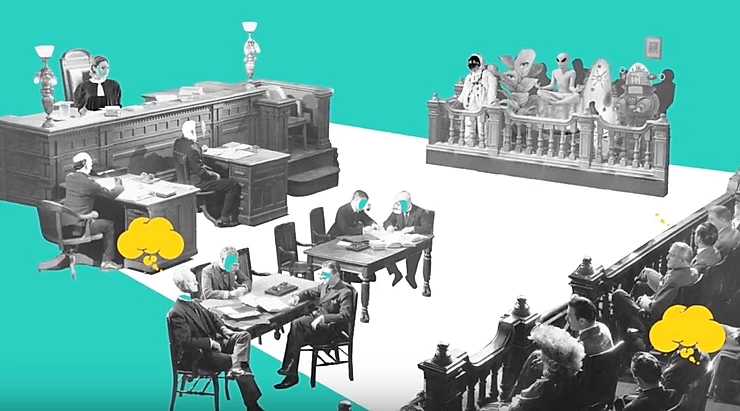
\includegraphics[height=\paperheight]{tribunal.png}}
%\section{\noindent\colorbox{shadecolor}
%	{\parbox{\dimexpr\textwidth-2\fboxsep\relax}{\textcolor{white}{Questions}}}}
%\usebackgroundtemplate{}


%-=-=-=-=-=-=-=-=-=-=-=-=-=-=-=-=-=-=-=-=-=-=-=-=
%	References:
%-=-=-=-=-=-=-=-=-=-=-=-=-=-=-=-=-=-=-=-=-=-=-=-=
\begin{frame}[t,allowframebreaks]{References}
\tiny
\bibliographystyle{apalike}
\bibliography{references}	
\end{frame}

\end{document}
